% Statistics assignment (English, university), with data tables and a tikz probability tree.
% Headings: "Question N" in bold with "[P marks]" at the right margin; parts (a), (b), ...
\documentclass[11pt,a4paper]{article}
\usepackage[T1]{fontenc}
\usepackage{lmodern}
\usepackage[margin=2.3cm,top=2.0cm,bottom=2.2cm]{geometry}
\usepackage{amsmath,amssymb}
\usepackage{siunitx}
\usepackage{booktabs}
\usepackage{caption}
\usepackage{tikz}
\usetikzlibrary{arrows.meta}
\usepackage{enumitem}

\setlength{\parindent}{0pt}
\setlist[enumerate,1]{label=(\alph*), leftmargin=2.2em, itemsep=0.35em, topsep=0.3em}
\newcommand{\question}[2]{\bigskip\par\noindent\textbf{Question #1}\hfill[#2 marks]\par\nopagebreak\smallskip}

\begin{document}

% ---- header ---------------------------------------------------------------------------
{\small STAT 2010 \textperiodcentered{} Introduction to Statistics \hfill School of Mathematical Sciences}\\[-0.4em]
\rule{\linewidth}{0.6pt}\\[0.5em]
{\Large\bfseries Assignment 5}\\[0.4em]
Submit by Friday 20 November 2026, 4 pm \hfill Total: 36 marks\\[0.3em]
{\small Calculators are allowed. Report intermediate results to at least four significant figures.}

% ---- Question 1 -----------------------------------------------------------------------
\question{1}{8}
Eight students were asked how many hours per week they study. The answers are in Table~1.

\begin{center}
\begin{tabular}{lcccccccc}
\toprule
Student & 1 & 2 & 3 & 4 & 5 & 6 & 7 & 8 \\
\midrule
Hours per week & 8 & 10 & 12 & 9 & 11 & 13 & 7 & 10 \\
\bottomrule
\end{tabular}
\captionof{table}{Weekly study time of eight students.}
\end{center}
\begin{enumerate}
  \item Find the sample mean and the median.
  \item Find the sample variance and the sample standard deviation.
  \item Compute the $z$-score of the student who studies 13 hours.
  \item Compute the coefficient of variation $s/\bar{x}$ as a percentage.
\end{enumerate}

% ---- Question 2 -----------------------------------------------------------------------
\question{2}{6}
A machine fills bottles. The filling volume is normally distributed with known standard deviation
$\sigma = \qty{6.0}{mL}$. A sample of $n = 36$ bottles has mean volume $\bar{x} = \qty{502.0}{mL}$.
\begin{enumerate}
  \item Construct a 95\% confidence interval for the true mean $\mu$.
  \item How wide is the 99\% confidence interval? ($z_{0.005} = 2.576$)
  \item How many bottles are needed so that the margin of error of a 95\% interval is at most
        \qty{1.0}{mL}?
\end{enumerate}

% ---- Question 3 -----------------------------------------------------------------------
\question{3}{8}
A manufacturer claims that its batteries last \qty{40.0}{h} on average. A consumer group tests
$n = 9$ batteries and finds a mean life of $\bar{x} = \qty{37.5}{h}$ with sample standard deviation
$s = \qty{4.5}{h}$. Assume the lifetimes are approximately normal. Use $t_{0.05,\,8} = 1.860$ and
$t_{0.025,\,8} = 2.306$.
\begin{enumerate}
  \item State the null and the alternative hypothesis for testing whether the batteries last
        \emph{less} than claimed.
  \item Compute the value of the test statistic.
  \item Decide at the $5\%$ significance level and state your conclusion in words.
  \item Construct a two-sided 95\% confidence interval for $\mu$. Is it consistent with your decision in (c)?
\end{enumerate}

% ---- Question 4 -----------------------------------------------------------------------
\question{4}{8}
Five measurements of the pair $(x, y)$ are given in Table~2.

\begin{center}
\begin{tabular}{lccccc}
\toprule
$x$ & 1 & 2 & 3 & 4 & 5 \\
$y$ & 2 & 3 & 5 & 4 & 6 \\
\bottomrule
\end{tabular}
\captionof{table}{Five measurements.}
\end{center}
\begin{enumerate}
  \item Compute $\bar{x}$ and $\bar{y}$.
  \item Find the least-squares regression line $\hat{y} = b_0 + b_1 x$.
  \item Predict $y$ for $x = 6$.
  \item Compute the correlation coefficient $r$ and the coefficient of determination $R^2$.
  \item Compute the residual of the point $(4, 4)$.
\end{enumerate}

% ---- Question 5 -----------------------------------------------------------------------
\question{5}{6}
A factory has two machines. Machine A makes 60\% of all items and machine B makes the other 40\%.
Of the items from A, 2\% are defective; of the items from B, 5\% are defective. The tree shows all
probabilities; $D$ means ``defective''.

\begin{center}
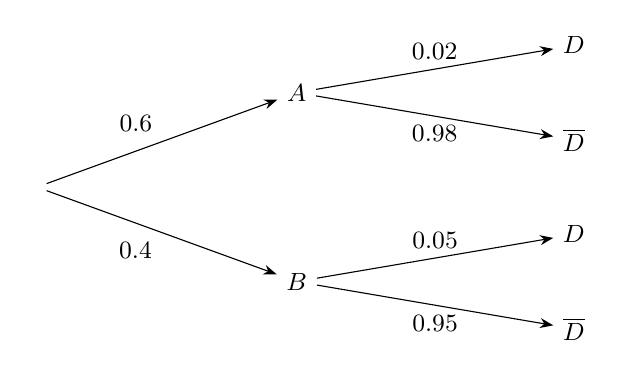
\begin{tikzpicture}[>=Stealth, xscale=1.1,
    every node/.style={font=\small}]
  \node (root) at (0,0) {};
  \node (A) at (3,1.2) {$A$};
  \node (B) at (3,-1.2) {$B$};
  \node (AD)  at (6.2,1.8)  {$D$};
  \node (AND) at (6.2,0.6)  {$\overline{D}$};
  \node (BD)  at (6.2,-0.6) {$D$};
  \node (BND) at (6.2,-1.8) {$\overline{D}$};
  \draw[->] (root) -- (A)   node[midway, above left]  {0.6};
  \draw[->] (root) -- (B)   node[midway, below left]  {0.4};
  \draw[->] (A) -- (AD)     node[midway, above]       {0.02};
  \draw[->] (A) -- (AND)    node[midway, below]       {0.98};
  \draw[->] (B) -- (BD)     node[midway, above]       {0.05};
  \draw[->] (B) -- (BND)    node[midway, below]       {0.95};
\end{tikzpicture}
\end{center}
\begin{enumerate}
  \item What is the probability that a randomly chosen item is defective?
  \item An item is found to be defective. What is the probability that it came from machine B?
  \item Two items are chosen independently at random. What is the probability that exactly one of them
        is defective?
\end{enumerate}

\end{document}
